% CRITERIA	(1 page)
	% ?Materials & Method
	% ?Datasets
	% ?Materials (sources)
	% ?Methods (reference and brief description)
	% ?Proposed approach: algorithm
	% ?Equations and formulas
%
Path planning is an active area of research due to the complexity of the problem and the need for a robust solution applicable to various environments. Many algorithms exist, but none of the proposed algorithms are capable of encompassing all the problem constraints for all environments \cite{sariff06}.

Existing path planning solutions include reactive motion planning algorithms, graph and probabilistic based motion planning, and optimization based planning \cite{waslanderI}. Each of these has advantages and disadvantages with regards to planning a route through a robot's environment. Reactive planning algorithms such as potential field and wavefront methods are simple in concept however these are local approach methods and do not consider dynamic constraints. Some are inherently susceptible to local minima, making them unacceptable for obstacle avoidance \cite{koren91}.

The wavefront method is designed to find the absolute shortest path, and as such will be used as the benchmark against which results from the suggested algorithm will be measured. It is expected that while the suggested algorithm will generate a longer path, the dynamic constraints will be satisfied, unlike the results of the wavefront solution.

Graph based planning offers a global approach. Graphs may be generated both deterministically (visibility graphs, cell decomposition, Voronoi diagrams), or randomly (probabilistic road maps). Established algorithms (such as Dijkstra's shortest path search) are used to extract the shortest path from the graph \cite{dijkstra59}. However dynamics of the robot are ignored in the generation of the graph, and this is detrimental to the criterion of path smoothness. Challenges also arise when there are restrictive obstacles such as narrow passages, however research in areas such as probabilistic road maps (PRMs) offers promising solutions \cite{hsu03}. Optimization based planning offers more confidence in finding a global optimum, however it is hindered by a lack of robustness: a poorly formulated problem may never converge \cite{waslanderIII}. It is also difficult to define obstacles.

In an effort to provide a simple method of avoiding obstacles and defining a path, the manipulator's configuration space will be discretized using a grid-based approach, and curve fitting techniques will be employed to find the ideal path. The configuration space of a robotic manipulator is a transformation of the manipulator's joint space to a two-dimensional Cartesian space. Defining the environment with a grid-graph may not be the most effective (cell decomposition offers greater efficiency \cite{lingelbach04}), however it provides a simple way to define obstacles as well as flexibility in representation. The grid will represent the configuration space for an articulated industrial robot. The grid cell size will define the computational resources required. A trade-off between resolution in the grid and computational efficiency must be made.

B\'{e}zier curves have been suggested to define the fitted curves generated by the genetic algorithm \cite{choi10}. B\'{e}zier curves provide smooth paths between two vectors, and while very effective for lower-dimensional problems, B\'{e}zier functions become very computationally expensive as the problem dimensionality increases. This paper therefore aims to use polynomial curve fitting in combination with genetic algorithms to optimize the curve. The curve will be optimized by minimizing distance, maximizing smoothness (minimizing jerk), and ensuring a safe passage around all obstacles. Genetic algorithms present an appealing approach for such complex optimization problems and offer good robustness as well \cite{zou12}.

The father of genetic algorithms, John Holland, modeled this machine intelligence technique after Darwin's Theory of Evolution, and the concept of ``survival of the fittest'' which he observed in nature. There are two natural learning epitomes available: the brain and evolution. Holland was inspired by the fact that the processes of natural evolution and natural genetics have become elucidated over decades of study in biology and molecular biology \cite{goldberg88}. The subtleties of the fundamental mechanisms of the brain, in contrast, are still shrouded in mystery. As such it seems clear to use the better understood model of genetic evolution as a platform for an optimization technique.

Research has already been done regarding the application of the parallel heuristic search method of genetic algorithms to curve fitting \cite{gulsen95,karr91,ismail08}. This paper builds upon that research. The goal is to find the coefficients of a polynomial function that will define a path with optimized path criteria. Thus each chromosome will contain a set of function parameters, labeled $\{P_3, \ldots, P_0\}$ in Equation \ref{eq:polyTraj}.

\begin{align} \label{eq:polyTraj}
	\phi = P_3*\theta^3 + P_2*\theta^2 + P_1*\theta + P_0
\end{align}

Testing will be performed by creating random environments containing arbitrarily placed objects. The algorithm will then plot a trajectory between a randomly defined start and end point. Many iterations of these tests will be performed in a variety of environments in order to accurately determine the effectiveness of this algorithm. The average path distance for each environment will be compared to the minimum distance as calculated by a Wavefront algorithm \cite{waslanderI}.

The wavefront algorithm is a deterministic algorithm which is capable of finding the shortest path between two points through a discretized environment. This will provide a ``gold standard'' which can be used to evaluate the performance of the genetic algorithm. The wavefront implementation used in this study permits  only 90 or 45 degree turns through the environment. A sample trajectory defined by a wavefront algorithm is presented in Figure \ref{fig:wfSol}. Since the genetic algorithm is a stochastic search, it will not result in an identical path twice. As such all results will be presented as averages and their associated distributions.

\begin{figure}[h]
	\centering
	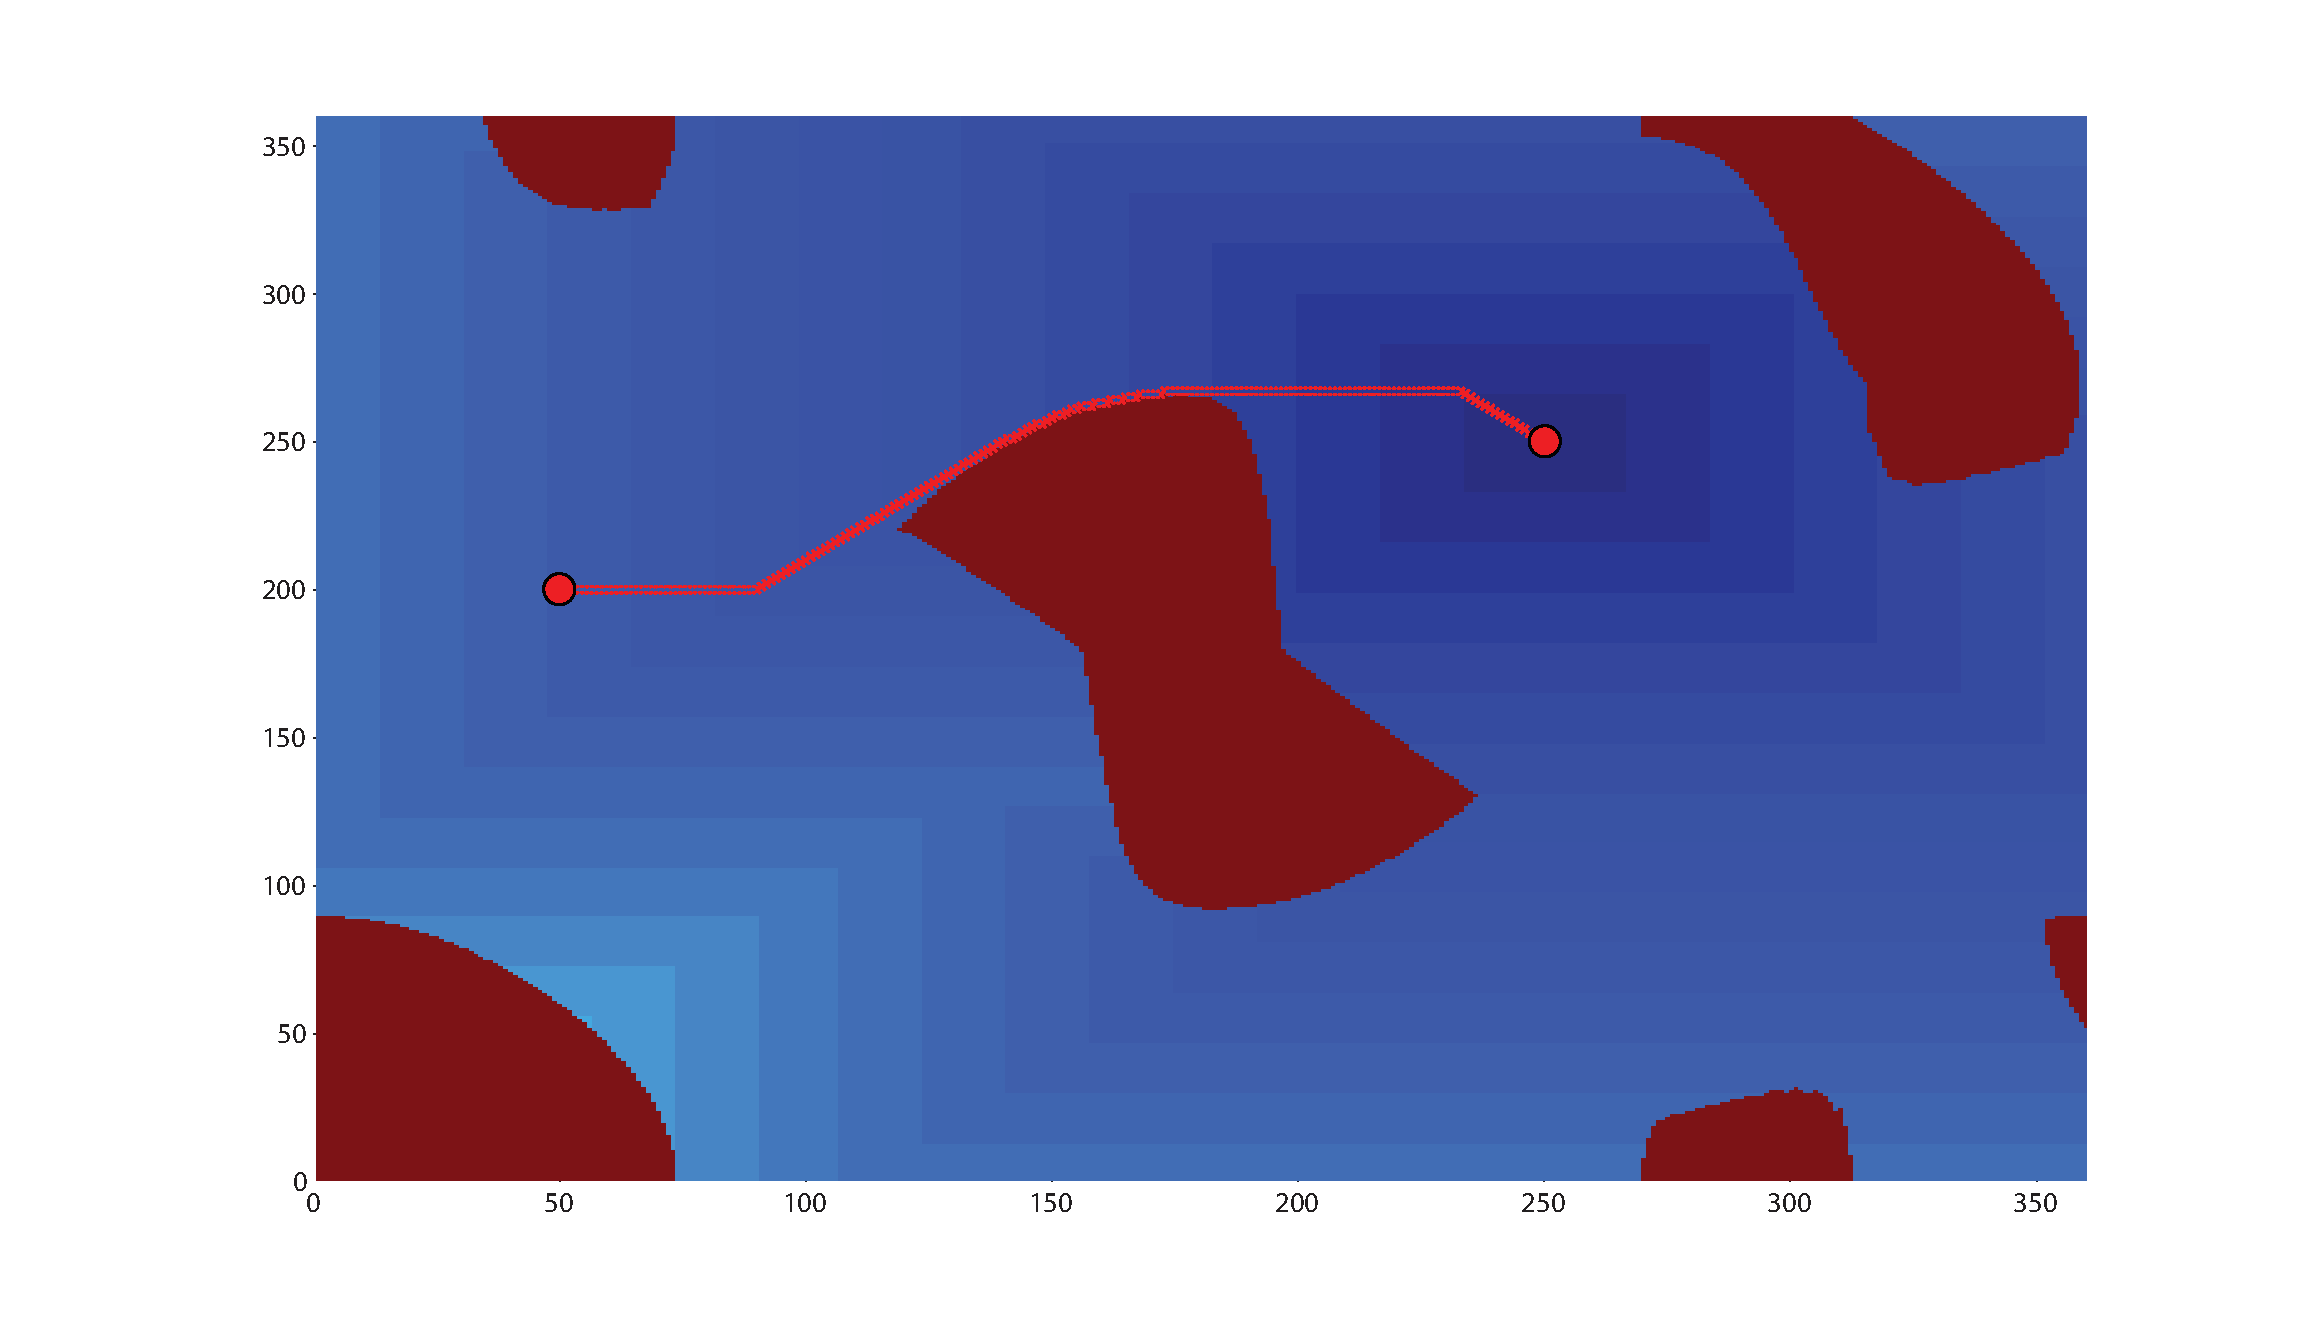
\includegraphics[width=\figWidth]{./figures/wavefrontSol.eps}
	\caption{The path as determined by the wavefront algorithm used to evaluate the performance of the genetic algorithm. The origin of the path is denoted by the darker blue, and the ``wave'' propogation is shown by increasingly light blue coloured cells.}
	\label{fig:wfSol}
\end{figure}

The result will be a global path planning algorithm functional in a static environment. Dynamic environments are possible with the proposed algorithm, however computational efficiency must be optimized in order to minimize the time required to find the solution. This new application offers a simple way to determine a path while taking into consideration all the defined path criteria.